%! program = pdflatex

%\documentclass[12pt,a4paper]{memoir} % for a long document
\documentclass[10pt,letter,final,article,twocolumn]{article} % for a short document
%\usepackage[left=0.25in,top=0.25in,right=0.25in,bottom=0.25in,nohead,nofoot]{geometry} 
\usepackage{titling,url}
\usepackage{graphicx}
\usepackage[numbers]{natbib}
% See the ``Memoir customise'' template for some common customisations
% Don't forget to read the Memoir manual: memman.pdf

\newcommand{\rpc}[1]{\emph{#1}}

\title{Minni: Minimalistic MapReduce}
\author{Athula Balachandran \\
{\tt abalacha@cs.cmu.edu}
\and
Wolfgang Richter \\
{\tt wolf@cs.cmu.edu}
\and
Erik Zawadzki \\
{\tt epz@cs.cmu.edu}}
\date{April 5, 2010} % delete this line to display the current date

%%% BEGIN DOCUMENT
\begin{document}

\pagenumbering{arabic}

\maketitle

\section{Introduction}
MapReduce~\citep{mapreduce08} is a distributed programming framework that facilitates the creating and execution of fault-tolerant data processing. The user can concisely write their entire program as two functions---the \emph{map} and \emph{reduce} functions---that the MapReduce run-time system distributes, schedules and executes. 

There have been many implementation of the MapReduce framework \citep{mochi,hadoop10,disco10,sphere09}. Of these, the most widely used is Hadoop. Hadoop was not designed to minimize memory use and as a result it has a large in-memory footprint. This prevent it from running on memory constrained systems, such as FAWN~\citep{fawn09}. Our project addresses this issue by identifying design decisions that are important to decreasing a MapReduce implementation's in-memory footprint. We have implemented some of these design decisions to produce a light-weight MapReduce architecture that can be used be memory constrained systems.

%MapReduce~\citep{mapreduce08}, which was introduced by Google, supports distributed computing on huge datasets on large clusters involving commodity hardware. The framework allows programmers to easily write applications that process these datasets in a reliable and fault-tolerant manner.  The basic implementation  comprises of two stages---\emph{map} and \emph{reduce}. This framework is inspired by the map and reduce functions that are commonly used in functional programming. The input data set is split into independent chunks and are parallel processed by the \emph{map} tasks. The output from this stage is then passed---potentially after an optional local stage called \emph{combine}---to the \emph{reduce} tasks. The framework abstracts all details like scheduling tasks, monitoring tasks, and re-executing of failed tasks. 

%The architecture typically consists of a master node and several worker nodes that store data as well as execute both \emph{map} and \emph{reduce} jobs assigned by the master. The fact that the worker nodes store data as well as process them has been used to come up with efficient scheduling techniques that take into account locality and enable minimization of network traffic.

%Several implementations of MapReduce are available \citep{mochi,hadoop10,disco10,sphere09}.  Most of the existing implementations of MapReduce try to minimize communication overhead between the worker machines. However, memory footprint is not an important consideration in many design decisions. This is of importance while designing MapReduce for systems like FAWN~\citep{fawn09}. In this project, we try to identify design possibilities that are key to decreasing memory footprint and we plan to re-implement a light weight MapReduce architecture that can be potentially be used by systems like FAWN.

\section{Previous Work}

The foundation for our implementation is the original description of MapReduce~\citep{mapreduce08}. While MapReduce is one of the best known distributed computing frameworks, there are other related architectures such as Dryad~\citep{dryad07} and parallel relational databases (see, for example, \citet{db210} and \citet{teradata10}) which are much more general than MapReduce.  In this project we will only focus on the MapReduce framework, but some of our design decisions (such as aggregation) are important for memory-constrained implementations of these other frameworks.
%Our implementation on top of FAWN~\citep{fawn09} introduces a particular constraint that the original MapReduce design did not consider: low memory.  
%In addition, FAWN uses flash storage as its principal storage medium which introduces another area for MapReduce research---the original MapReduce design assumes a storage medium of hard drives.  

A recent paper by \citet{yu2009distributed} evaluates some of the different design choices for MapReduce and MapReduce-like systems. One of key decisions that they identify is aggregation strategy.  They show that the aggregation strategy used by Hadoop and the original MapReduce is empirically inferior to a competing method based on hashing which is used by major commercial databases (\emph{e.g.} DB2~\citep{db210} and Oracle~\citep{oracle10}). They also point out that the aggregation method has a significant impact on the memory footprint of jobs. This is particularly important for our project and we will discuss this issue later.

Other research has shown that techniques such as merging the MapReduce stages~\citep{barrier10}, and dynamically prioritizing resource usage~\citep{sandholm09} offer substantial performance benefits over the standard MapReduce design. We adopt both of these techniques in our implementation.

There are several existing MapReduce implementations, such as Disco~\citep{disco10}, Hadoop~\citep{hadoop10}, and Sector and Sphere~\citep{sphere09}. These implementations differ from our own since they do not target low-memory, but we did use these other implementations---Hadoop in particular---as a guide to identify important design decisions. In addition to these general MapReduce implementations there are also a number of hardware-specific implementations that target Cell Broadband architecture~\citep{rafique09} and multicore systems~\citep{chu06}. These implementations have an orthogonal goal to our own: we want to handle large arrays of heterogenous computers that may have limited memory.

%Finally, we can take advantage of FAWN's energy efficiency which is an active area of research with MapReduce as reflected in Gordon~\citep{gordon09},  and work analyzing MapReduce traces for future energy efficiency goals~\citep{chen10}.

\section{Architecture}
\label{sec:arch}
\begin{figure}[htbp]
\begin{center}
\resizebox{\columnwidth}{!}{
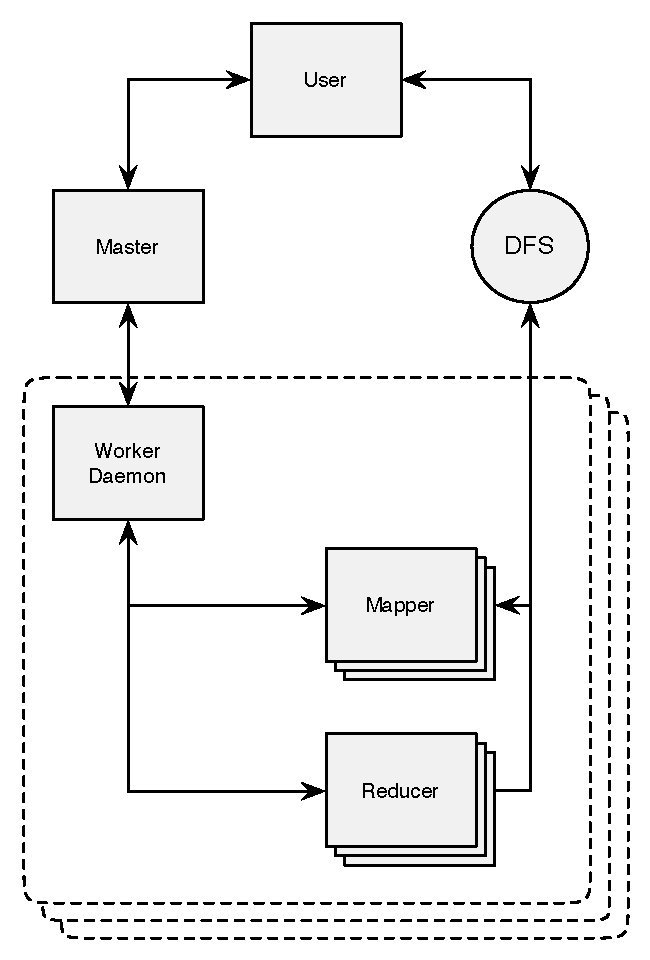
\includegraphics{Architecture.pdf}
}
\caption{The major components found in our architecture.}
\label{fig:arch}
\end{center}
\end{figure}


\begin{figure}[htbp]
\begin{center}
\resizebox{\columnwidth}{!}{
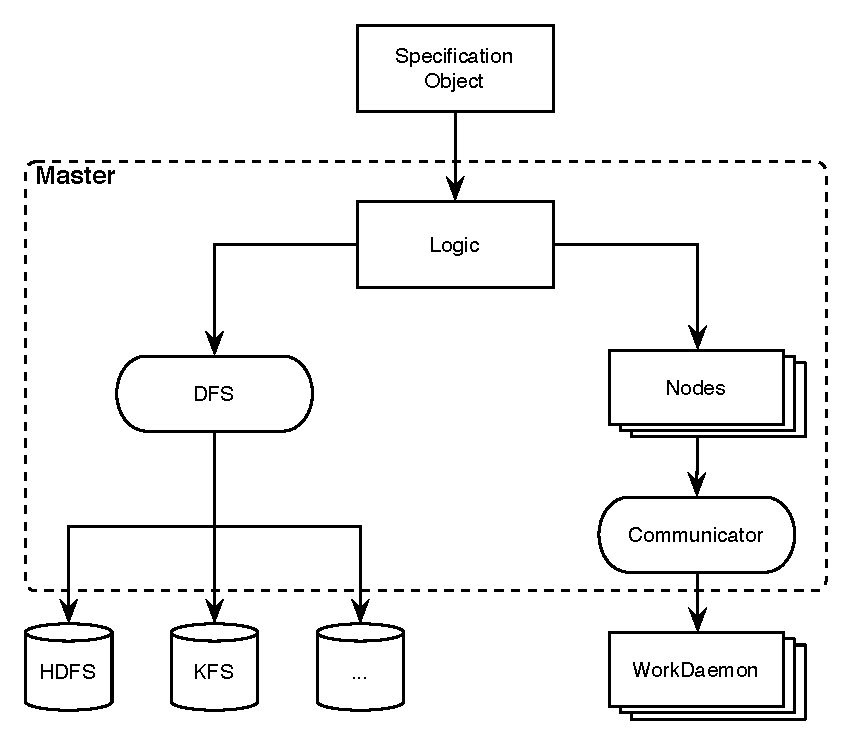
\includegraphics{master.pdf}
}
\caption{A diagram of the master system and the components that it communicates with.}
\label{fig:arch}
\end{center}
\end{figure}


Our proposed architecture is shown in Figure~\ref{fig:arch}. We first describe the major difference between our proposed architecture and the architecture suggested in prior implementations of MapReduce. We then explain our architecture and the RPCs it uses to communicate by taking the reader through the running of a typical MapReduce job. We finish this section by describing our mechanisms for tolerating faults and summarize the RPCs used in our architecture.

\subsection{Main difference}

There are three major differences between our implementation and standard MapReduce. The first is the introduction of a local manager process called the \emph{WorkDaemon} (WD) that manages a single node. The second difference is that we use the \emph{Accumulator-PartialHash} (APH) aggregation scheme, as described in \citet{yu2009distributed}.

\subsubsection{WorkDaemon}

The first major difference is the WD that sits on each node that mediates all communication between the master and the worker---including RPCing intermediate key/values to the reducers. This has some advantages and disadvantages.

There are three advantages to this approach. The first is that mapper threads can free system resources by closing immediately upon completion. This is especially important in systems where memory is scarce. This property has a secondary advantage: it entirely removes a failure case. Jobs no longer need to be rerun if mappers crash after completion since the daemon is responsible for all RPC with the reducers. Additionally, since worker communication is centralized by the WD we can reduce network overhead by batching messages.

The principle disadvantage of the WD approach is that the WD takes the node down when it crashes. In our failure model a node is removed from the MapReduce pool if the WD crashes. However, since the WD is isolated from the user's code and data we expect this to be a somewhat rare event.

\subsubsection{Accumulator-PartialHash}

The second major difference is the adoption of the APH aggregation scheme. \citet{yu2009distributed} describes the original MapReduce approach as the \emph{FullSort} method: all the records are gathered in memory and sorted by intermediate key immediately following the map phase\footnote{If there are too many key-value pairs to store in memory then they are sorted externally.}. This method has two principle disadvantages: it may be memory intensive (unless we always sort externally in which case it is slow), and requires every key-value pair to be present in memory before sorting. 

 APH aggregation alleviates both these problems. APH essentially combines the sort phase an initial reduction. Each task has a hashtable that maps keys to partial aggregation objects (PAOs).These PAOs, intuitively, are some sufficient description of an incomplete aggregation such that:
\begin{itemize}
 \item a new key-value pair can be \emph{added} to the PAO to yield a new PAO (\emph{i.e.} $(k,p^t) = (k,p^{t-1}) + (k,v^t)$);
 \item two PAOs can be \emph{merged} to form a new PAO (\emph{i.e.} $(k,p^s) = (k,p^q) \oplus (k,p^r)$).
\end{itemize}
When a new object (either a value or a PAO) with a particular key is give to a reducers task, the task adds it to or merges it with the appropriate PAO in the hashtable. The PAO can be understood as being the sufficient description of a suspended reducer. The user describes this reduction with an initialization function, addition function and merger function, and serialization routines\footnote{We would provide some serialization support for STL containers in a polished library.} for this PAO instead of a single reduce function.

This new formulation yields some immediate advantages: if the PAO grows less than linearly in the number of key-value pairs then the memory used by a collection of PAOs will be less than then memory used by the complete list of key-value pairs. Indeed, for many examples like $k^{th}$-order statistics and word count the PAO is constant size. In other cases like grep the size of the PAO---represented internally by, say, a list of lines that match the pattern---might actually grow linearly with the size of the input but with a very small constant.

Additionally, by evicting any PAO object that either 1) is too large or 2) has a hash-value with many collisions, then we can guarantee an upper bound on the memory footprint for a reducer task. (The \emph{eviction policy}---the policy that selects PAOs to write to disk---must balance between evicting early to save memory and evicting late to maximize data compression).  

A second advantage of this approach is that we can start reducers immediately after at least one mapper finishes. This eliminates time spend waiting for key-value pairs to gather. Finally, since we don't sort. APH aggregation only requires key equality tests, rather than order comparisons. This means the programmer can avoid having to define spurious ``greater-than'' notions.

Finally, the use of PAOs suggests some useful design modifications for the mapper. In the traditional MapReduce system, each mapper writes intermediate key-value pairs to local disk. These key-value pairs might be shipped to the reducers as-is or merged prior to transmission in a combiner phase. The combiner phase is a local reduce that reduces the size of the transmitted data. In our scheme, rather than writing the intermediate key-values to files at all, we have a per-mapper local reducers that aggregates the key-value pairs into PAOs. These PAOs are then written to disk, and may be more completely combined in a per-node local reducer. 

This achieves the same end result as the original combiner phase, but may be better in terms of memory, performance and disk usage. The PAOs that result from the per-mapper can be much smaller than total list of key-value pairs, so it might be possible to keep them all in a small amount of memory rather than constantly buffering and writing key-value pairs to disk.

This formulation also has some disadvantages. Chief among these, some users may have a MapReduce formulation for their problem that assumes that the key-value pairs are initially sorted and rely on this fact to process them in sequence. We are breaking this for our prototype and explicitly assuming that key $k_i$ may be processed entirely independently from the processing of key $k_j$. In a full-featured release version of this program we would likely want to provide the user with a way of insisting that the key-value pairs be sorted, but we will not initially include this feature.

We initially worried that the PAOs might also obfuscate errors. For example, in the original MapReduce paper, key-value pairs could be flagged as `bad' and skipped if multiple reduce or map tasks fail on them. While we can still mark a record that causes repeated problems when we try to add it to a PAO as `bad', it is less clear what should be done if merging PAOs fails. Scrapping work and rerunning the tasks that generated the PAO could solve the problem if there was some order-dependent error, but what do we do if we just can't seem to get some PAOs to merge?

We believe that  the original intent of the bad-records was primarily to guard against anomalous data, and not logic problems with the user code. We can still provide reliability in the face of anomalous data by recording the last key-value pair that was successfully added to a PAO in the initial reduce, and some robustness to logical errors by rerunning PAO calculations, but we will  pass any repeated merger errors to the user---such errors represents a serious logical problem that is likely independent from \emph{where} the task was run. Additionally, if we have consistent problems merging two user-defined objects, this casts serious doubt on the validity of the user's code.

We feel that our design decision to use APH aggregation is reasonable for a MapReduce implementation that is primarily intended for memory-constrained systems.

\subsection{Typical Use}

\begin{figure}[htbp]
\begin{center}
\resizebox{\columnwidth}{!}{
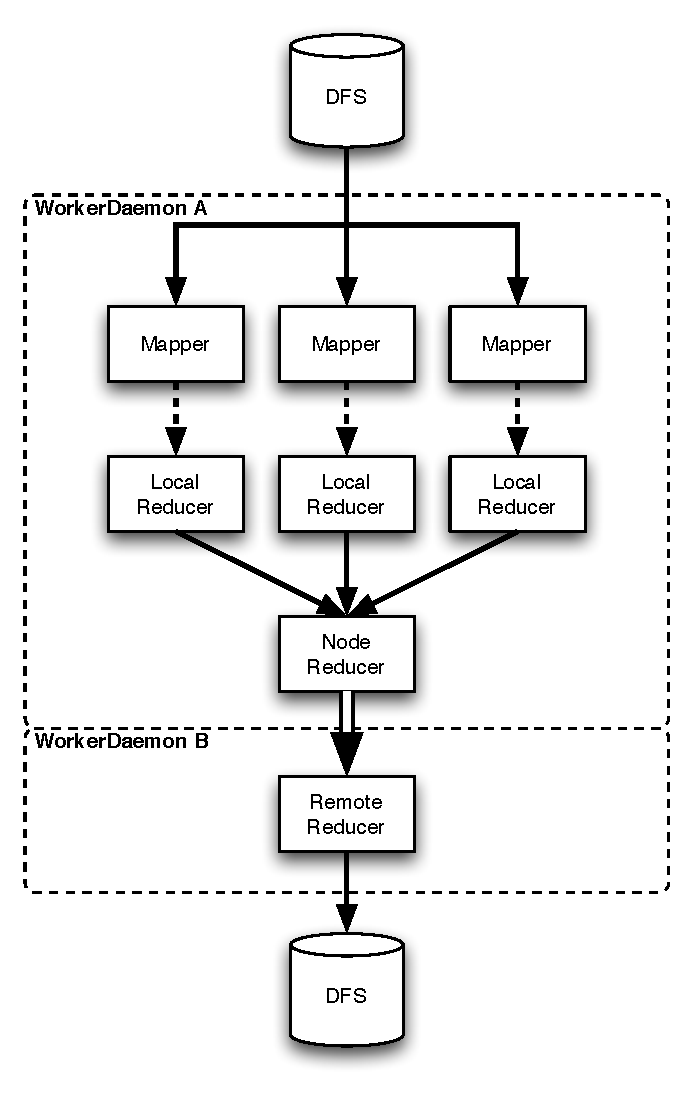
\includegraphics{data_flow.pdf}
}
\caption{An example of how data flows through our system.}
\label{fig:flow}
\end{center}
\end{figure}


So how does a typical MapReduce job look on this system? The sequence is initiated by the user when he contacts the master process and submits a MapReduce job using the \rpc{SubmitJob} RPC, which the user will block on.  In the initial version of our system we will assume that there is a single well-known master that is always available and that failures of the master are catastrophic. The details for the job are provided in the form of a \emph{specification object}. The user provides in the specification the name of the shared object library that contains the user code (the \emph{map} function and all the PAO operations), the location on the DFS of the input data, and the DFS location to write all the output. The user will pass this code to our program by implementing known functions and dynamically linking their object files into our code.

After receiving the initial message the master requests that the WorkDaemon on each node start \emph{mapper} threads with a \rpc{StartMapper} call. The master will prefer to place \emph{map} jobs on nodes that have a replicated copy of the appropriate split of the input data and nodes that are not busy.  We assume in this phase of the work that the user has access to the complete cluster and that the current MapReduce job is the only job running on the system. Later iterations of our work will have to include interactions with a cluster resource manager. We also currently assume that the WDs are already running on the worker nodes.

The WD, upon receipt of a \emph{map} work request, spawns a new \emph{mapper} TBB task for each request it gets. Because the WD never delays or rejects any work request the master is completely responsible for work scheduling (the master maintains a tentative queue for each WD). The \rpc{StartMapper} call includes a chunk ID for the DFS. For now, we will assume that each chunk belongs to a single file and that we do not have to worry about the boundaries of multi-chunk files---\textit{e.g.} if a text document spans two chunks a word does not start in one block and end in another.

While mapping the input key-value pairs the mapper task also performs a  \emph{per-mapper local reduction}. To do this the mapper maintains a hashtable of PAOs---one for each key. When an input key-value pair has been mapped to an intermediate key-value the mapper task adds it to the appropriate PAO. Upon termination of the mapper the resulting PAOs are written to local disk. 

Upon termination the mapper task informs the WD that it is done and what files it produced. The WD can start an optional \emph{per-node local reducer}. The master occasionally polls the WDs for status changes, and upon receipt of one of these RPCs the WD will list all finished (or dead) mappers. 

When it learns that some mappers are done, the master initiates new \emph{final reducer} tasks with a \rpc{StartReducer} call. Whenever a WD informs the master that it has some new PAOs to read, the master passes this information on to the appropriate \emph{final reducers} with an \rpc{ReportData} call. If the PAOs  are local then the \emph{final reducer} can read them right from disk. If not, then the key/values are requested directly from the remote WD with a \rpc{SendData} call. The WD is responsible for tracking the state of all transmissions and collecting of the required PAOs for its final reducers. The \emph{final reducer} starts executing the user's \emph{merge} code as soon as it has collected at least two PAOs.

While running the user's code the \emph{reducer} thread writes the final key-PAO pairs to a temporary local file. Upon completion the \emph{final reducer} writes this local file to the DFS and reports to the WD. The WD forwards this to the master when polled by the \rpc{ReportWorkComplete} call.

We have summarized this data flow in Figure~\ref{fig:flow}

\subsection{Fault Tolerance}
The above process needs to be resilient to machines and threads failing. We will tolerate worker nodes, worker tasks, and WorkDaemons crashing. We will not tolerate the master failing.

We use a polling model to keep track of the dispatched jobs. The master polls WD to see if any of the active jobs have finished or failed. Whenever a mapper or a reducer task is working, the WD checks its running status to ensure that it has not terminated before reporting that it has completed its work.

If a job dies unexpectedly then the master will reschedule it. Notice that because the WD is responsible for sending data to the \emph{final reducers}, we do not need to notify any \emph{final reducers} about failed \emph{mappers}. 

If the entire node goes down (\textit{i.e.} the WD has not checked in for a while), then the master sends a \rpc{Kill} to the WD for all of its jobs, then \rpc{ReportFail}'s any reducer that are still waiting for PAOs from that node. Notice that since we ensure that all or no PAOs from a \emph{final reducer}, a node crash cannot leave us with a case where we have used some but not all of a \emph{initial reducer's} PAOs. Finally, the master reschedules all work on the downed node.

%\subsection{RPC calls}
%
%Here is a summary of the RPC calls used in our system:
%
%\begin{table}[htdp]
%\caption{Stored procedures on the master.}
%\begin{center}
%\begin{tabular}{|l|l|}\hline
%\textbf{Procedure} & \textbf{Arguments}\\\hline
%\rpc{SubmitJob} & SpecObject\\\hline
%\end{tabular}
%\end{center}
%\label{tab:master_rpc}
%\end{table}%
%
%\begin{table}[htdp]
%\caption{Stored procedures on the worker daemon}
%\begin{center}
%\begin{tabular}{|l|l|}\hline
%\textbf{Procedure} & \textbf{Arguments}\\\hline
%\rpc{StartMapper} & JobID, JobProperties\\
%\rpc{StartReducer} & JobID,  JobProperties\\
%\rpc{ReportData} & \\
%\rpc{ReportFail} & Mapper IP, Mapper JobID\\
%\rpc{SendData} & JobID, Key\\\hline
%\end{tabular}
%\end{center}
%\label{tab:worker_rpc}
%\end{table}%



\section{Evaluation}
In our evaluation section we are primarily interested in two things: first, do we actually have a smaller in-memory footprint than Hadoop? Secondly, how quickly do similar MapReduce jobs take Hadoop and Minni?
\subsection{Memory Profile}
\subsection{Performance}


\bibliographystyle{plainnat}
\bibliography{references}


\end{document}
